%% appendix/B-simulation-methodology.tex
%% Appendix B: Simulation Methodology
%% Describes the seeds, sample sizes, trial counts, and reproducibility
%% conventions used across the eight notebooks.

\section{Simulation Methodology}\label{app:simulation}

\paragraph{Single-realization Marchenko-Pastur companion plot.}
The varying-aspect-ratio figure in Section~\ref{subsec:scm-highdim} (Figure~\ref{fig:mp-varying-c}) pools eigenvalues from many independent realizations of \(\Sigmahat_n\) to make the limiting Marchenko-Pastur shape sharp. For comparison, Figure~\ref{fig:mp-bulk-single} below shows the histogram of a \emph{single} realization at \(p = 500\), \(n = 1000\) (\(y = 1/2\)). Even one realization is already enough for the empirical eigenvalue distribution to match the limiting Marchenko-Pastur density visually.

\begin{figure}[H]
  \centering
  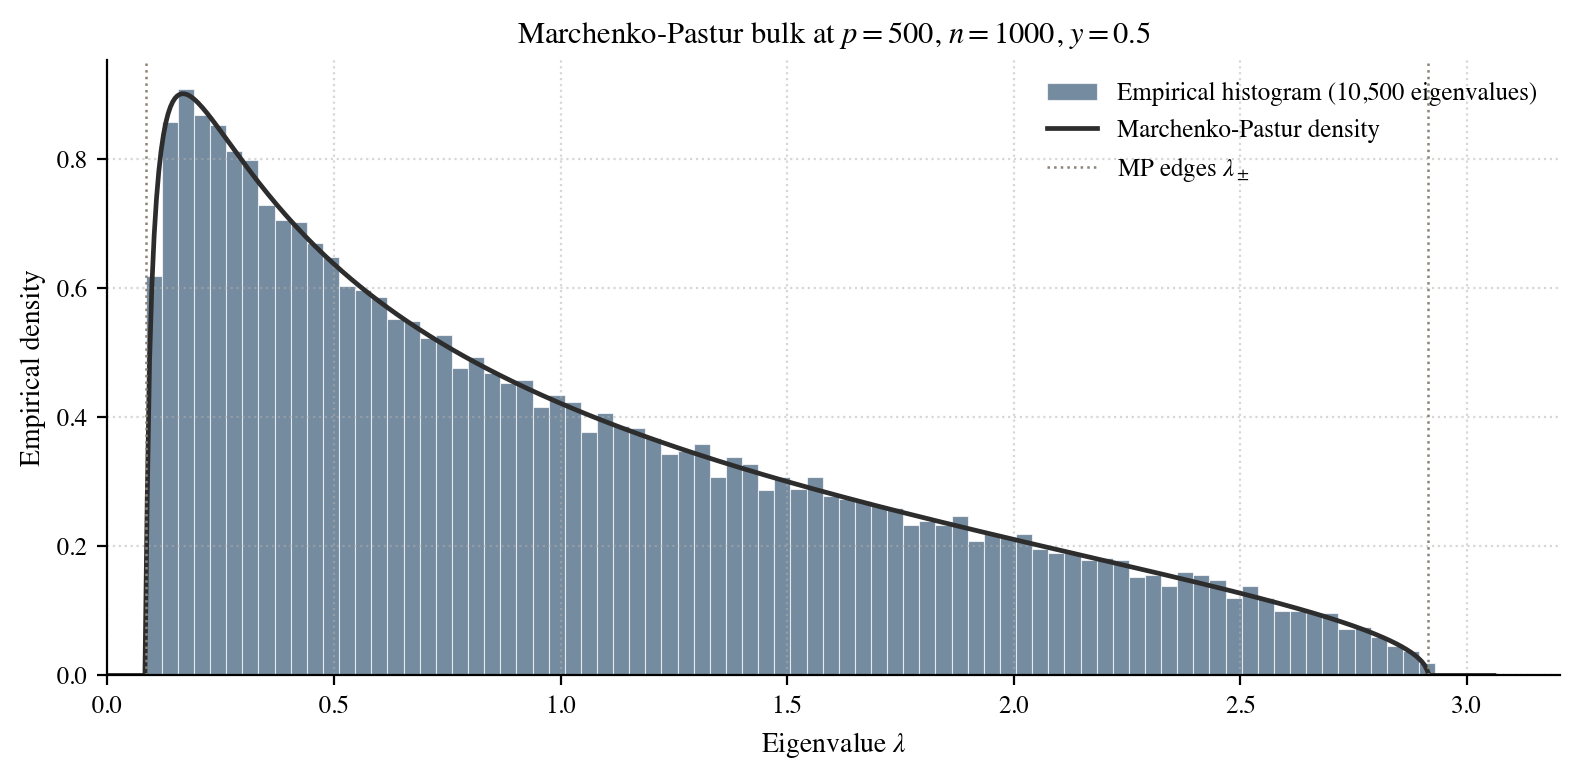
\includegraphics[width=0.82\textwidth]{figures/mp_bulk_with_density.png}
  \caption{Single-realization Marchenko-Pastur fit at \(p = 500\), \(n = 1000\) (\(y = 1/2\)). The histogram of all \(500\) eigenvalues from one draw of \(\Sigmahat_n\) closely matches the \(\MP_{1/2}\) density. The dotted lines mark the support edges \(\lambda_\pm = (1 \pm \sqrt{y})^2 \approx 0.086,\, 2.914\). Companion to Figure~\ref{fig:mp-varying-c} in Section~\ref{subsec:scm-highdim}. Generated by \texttt{notebooks/03\_section3\_demos.py}.}
  \label{fig:mp-bulk-single}
\end{figure}


\todo{Content to fill in:

B.1 General reproducibility conventions.
- All notebooks use Python 3, with \texttt{numpy}, \texttt{matplotlib}, and
  \texttt{scipy.stats}.
- Random number generation: \texttt{rng = np.random.default\_rng(seed)},
  with explicit \texttt{seed} at the top of every notebook.
- Eigendecomposition: \texttt{np.linalg.eigh} on symmetric inputs; the top
  eigenpair is taken as \texttt{evals[-1]}, \texttt{evecs[:, -1]}.
- Plot styling: shared helper module \texttt{notebooks/thesis\_style.py}
  applies the six-color palette and sans-serif math labels.

B.2 Per-notebook parameter table.
- Notebook 01 (LLN/CLT demos): \(n \in \{100, 1000, 10000\}\), 500 trials.
- Notebook 02 (Wishart and repulsion): \(n = 100\), \(p = 2\), 5000 trials.
- Notebook 03 (fixed-dim fluctuations): \(n = 500\), 5000 trials, both
  \(\Sigma = I_2\) and \(\Sigma = \diag(1, 2)\).
- Notebook 04 (Marchenko-Pastur \& TW): \(n = 1000\), \(y = 1/2\), 1 trial
  for bulk density, 1000 trials for top eigenvalue.
- Notebook 05 (spiked eigenvalues, BBP): \(y = 1/2\), \(n \in \{100, 200,
  400, 800, 1200\}\), 200 trials per \(n\), \(\alpha \in \{1.4, 2.5\}\).
- Notebook 06 (fluctuation Q-Q): \(n = 1200\), \(y = 1/2\), 500 trials,
  \(\alpha = 2.5\).
- Notebook 07 (eigenvector overlap): \(n = 1200\), \(y = 1/2\), 500 trials,
  \(\alpha \in \{1.4, 2.5\}\).
- Notebook 08 (spectral clustering toy): two-class Gaussian mixture,
  \(n = 600\) per class, \(p \in \{50, 200\}\).

B.3 Numerical caveats.
- For the strong-spike fluctuation Q-Q plot, we standardize empirically
  (subtract sample mean, divide by sample standard deviation) because the
  exact variance \(\sigma_{\alpha, y}^2\) requires constants from
  \citet[Thm.~11.11]{YaoZhengBai2015}.
- For the weak spike, we do not attempt an exact Tracy-Widom fit because
  the finite-sample centering and scaling constants are delicate; we report
  the qualitative shape of the histogram and defer the rigorous fit to
  future work.
- The realized aspect ratio \(p/n\) differs from the target \(y\) when
  \(yn\) is not integer; figures use the realized ratio in the bulk-edge
  formula \((1 + \sqrt{p/n})^2\) for consistency.}

\clearpage
